\documentclass[12pt,a4paper,twoside]{book}
% Language setup for Greek and English
\usepackage[english,greek]{babel}
\usepackage[utf8]{inputenc}
\usepackage[T1,LGR]{fontenc}
% Font setup
\usepackage{fontspec}
\setmainfont{Linux Libertine O}[Scale=0.9]
\setsansfont{Linux Biolinum}[Scale=0.9]
\setmonofont{DejaVu Sans Mono}[Scale=0.9]
% Other necessary packages
\usepackage{enumitem}
\usepackage{graphicx}
\usepackage{amsmath}
\usepackage{makeidx}
\usepackage{multicol}
\usepackage{multirow}
\usepackage{hanging}
\usepackage{adjustbox}
\usepackage{amssymb}
\usepackage{stackengine}
\usepackage{ifthen}
\usepackage{array}
\usepackage{tcolorbox}
\tcbuselibrary{skins,breakable}
\usepackage{minted}
\usepackage{listings}
\usepackage{parskip}
\usepackage{float}
\usepackage{subcaption}
\usepackage{xcolor}
\usepackage{cancel}
\usepackage{pdfpages}
\usepackage{titlesec}
% Page & text layout
\usepackage{geometry}
\geometry{
   a4paper,
   top=2.5cm,
   bottom=2.5cm,
   left=2.5cm,
   right=2.5cm
}
% Headers & footers
\usepackage{fancyhdr}
\pagestyle{fancyplain}
\fancyhf{} % Clear all header/footer fields

% Define plain style for chapter pages and TOC
\fancypagestyle{plain}{%
    \fancyhf{} % Clear all header/footer fields
    \renewcommand{\headrulewidth}{0pt} % Remove header rule
    \renewcommand{\footrulewidth}{0pt} % Remove footer rule
}

% Define TOC style with specific headers
\fancypagestyle{tocstyle}{%
    \fancyhf{} % Clear all header/footer fields
    \fancyhead[LE]{\thepage}
    \fancyhead[CE]{\leftmark}
    \fancyhead[CO]{\rightmark}
    \fancyhead[RO]{\thepage}
    \renewcommand{\headrulewidth}{0pt}
}

% Redefine \tableofcontents to use tocstyle
\let\oldtableofcontents\tableofcontents
\renewcommand{\tableofcontents}{%
    \clearpage
    % First page of TOC should be empty
    \thispagestyle{empty}
    \pagestyle{tocstyle}
    \oldtableofcontents % chktex 1
    \clearpage
    \pagestyle{fancy}
    % Regular pages header settings
    \fancyhead[LE]{\thepage} % Left header on Even pages: Shows page number
    \fancyhead[CE]{\leftmark} % Center header on Even pages: Shows chapter name (stored in \leftmark)
    \fancyhead[RE]{ΚΕΦ. \thechapter} % Right header on Even pages: Shows "ΚΕΦ." followed by chapter number % chktex 12

    \fancyhead[LO]{\thesection} % Left header on Odd pages: Shows current section number
    \fancyhead[CO]{\rightmark} % Center header on Odd pages: Shows section name (stored in \rightmark)
    \fancyhead[RO]{\thepage} % Right header on Odd pages: Shows page number

    \renewcommand{\headrulewidth}{0.4pt} % Sets thickness of the horizontal line below the header

    % Redefine chapter mark to remove "Chapter" prefix
    \renewcommand{\chaptermark}[1]{\markboth{#1}{}}
    % Redefine section mark to use section title only
    \renewcommand{\sectionmark}[1]{\markright{#1}}
}

% Make table of contents use plain style
\addtocontents{toc}{\protect\thispagestyle{plain}}

% Hyperlinks
\usepackage{hyperref}
\usepackage{bookmark}                                       % Add this line to fix the hyperref warnings
\hypersetup{
    colorlinks=true,
    linkcolor=blue,
    citecolor=blue,
    filecolor=blue,
    urlcolor=cyan,
    unicode,
    pdftitle={Pet-à-vet},
    pdfsubject={Αναφορά Εργασίας},
    pdfborderstyle={/S/U/W 1},                              % Underline links
}
\usepackage{tikz}
\usetikzlibrary{positioning, shapes.geometric, arrows.meta}
\usepackage{pgfplots}
\pgfplotsset{compat=1.18}
\usetikzlibrary{calc,arrows.meta,positioning}

\definecolor{customRed}{HTML}{FF5F5A}                       % using hexadecimal
\definecolor{customYellow}{HTML}{FFBE2E}                    % using hexadecimal
\definecolor{customGreen}{HTML}{2ACA44}                     % using hexadecimal
\definecolor{customPurple}{HTML}{C477DB}                    % using hexadecimal
\definecolor{customBlue}{HTML}{052538}                      % using hexadecimal
\definecolor{customLightBlue}{HTML}{60ADEC}                 % using hexadecimal
\definecolor{customGray}{HTML}{A0A0A0}                      % using hexadecimal
\definecolor{customBlack}{HTML}{000000}                     % using hexadecimal

% Define a lighter gray for background and darker colors for text
\definecolor{customBgGray}{HTML}{E0E0E0}         % Light gray background
\definecolor{customCodeRed}{HTML}{C92A2A}        % Darker red
\definecolor{customCodeYellow}{HTML}{E67700}     % Darker yellow/orange
\definecolor{customCodeGreen}{HTML}{087F23}      % Darker green
\definecolor{customCodePurple}{HTML}{7B1FA2}     % Darker purple
\definecolor{customCodeBlue}{HTML}{1976D2}       % Darker blue
\definecolor{customCodeBlack}{HTML}{1A1A1A}      % Lighter black

\lstdefinestyle{myPythonStyle}{
    language=Python,                                            % Set the language to Python
    backgroundcolor=\color{customBgGray},                       % Background color
    basicstyle=\color{customCodeBlack}\ttfamily\footnotesize,   % Basic font style, size, and color
    keywordstyle=\color{customCodePurple}\bfseries,             % Style for general keywords
    keywordstyle=[2]\color{customCodeYellow}\bfseries,          % Style for specific keywords
    commentstyle=\color{customCodeGreen}\itshape,               % Style for comments
    stringstyle=\color{customCodeGreen},                        % Style for strings
    identifierstyle=\color{customCodeBlue},                     % Style for identifiers
    morekeywords={self, None, True, False, format, abs,
                as, pass, return, if, elif, else, for,
                range, while, try, except, with, lambda,
                yield, global, nonlocal, assert, del,
                raise, in, is, and, or, not},                   % Additional keywords
    morekeywords=[2]{os, graphviz, Digraph, collections,
                    deque, math, tabulate},                     % Define 'import' and 'from' as additional keywords
    % procnamekeys={def,class},                                 % Highlight function and class names
    showstringspaces=false,                                     % Don't show spaces in strings
%
    breaklines=true,                                            % Automatically break long lines
    breakatwhitespace=false,                                    % Break lines at any character
    % prebreak=\textbackslash,                                  % Character for breaking lines
    postbreak={\space},                                         % Character for breaking lines
    breakautoindent=false,                                      % Indentation after line break
    breakindent=0pt,                                            % Indentation before line break
    resetmargins=true,                                          % Reset margins after line break
    keepspaces=true,                                            % Keep spaces in the code
    showspaces=false,                                           % Don't show spaces
    columns=flexible,                                           % Column format
%
    numbers=left,                                               % Line numbers on the left
    numberstyle=\small\color{customBgGray},                     % Style for line numbers
    % numwidth=4em,                                             % Width allocated for line numbers
    stepnumber=1,                                               % Step between line numbers
    numbersep=8pt,                                              % Distance of line numbers from code
    xleftmargin=1.5em,                                          % Match the numwidth
    tabsize=4,                                                  % Size of a tab
    captionpos=t,                                               % Position of the caption (t for top)
    firstnumber=auto,                                           % Continue line numbering from previous listing
    aboveskip=0em,                                              % Remove external spacing
    belowskip=0em,                                              % Remove external spacing
    frame=none,                                                 % Add top and bottom rules only
    framerule=0pt,                                              % Make the rules invisible
    rulecolor=\color{customBgGray},                             % Color of the frame (if enabled)
    framesep=2pt,                                               % Add internal padding
    % framexleftmargin=1em,                                     % Add internal left margin
    % framexrightmargin=1em,                                    % Add internal right margin
    escapeinside={\(*@}{@*\)},                                  % For escaping characters
    morecomment=[l]{\#},                                        % Define comment style
    morestring=[b]',                                            % Define string style with single quotes
    morestring=[b]",                                            % Define string style with double quotes % chktex 18
    literate={
        {``}{{\textquotedbleft}}2
        {''}{{\textquotedbright}}2
        {`}{{\textquoteleft}}1
        {'}{{\textquoteright}}1
        {_}{{\_}}1
    },
}

\lstdefinestyle{myCStyle}{
    language=C,
    backgroundcolor=\color{customBgGray},                       % Background color
    basicstyle=\color{customCodeBlack}\ttfamily\footnotesize,   % Basic font style
    keywordstyle=\color{customCodePurple}\bfseries,            % Style for keywords
    keywordstyle=[2]\color{customCodeYellow}\bfseries,         % Style for additional keywords
    commentstyle=\color{customCodeGreen}\itshape,              % Style for comments
    stringstyle=\color{customCodeGreen},                       % Style for strings
    identifierstyle=\color{customCodeBlue},                    % Style for identifiers
    morekeywords={void, int, char, float, double, long, short, signed, unsigned,
                  const, static, extern, volatile, register, auto, struct, union,
                  typedef, enum, sizeof, break, continue, goto, return, if, else,
                  switch, case, default, for, while, do, pid_t, sem_t},
    morekeywords=[2]{stdio.h, stdlib.h, string.h, math.h, time.h, ctype.h,
                     unistd.h, semaphore.h, sys/mman.h, sys/wait.h, fcntl.h,
                     printf, fprintf, perror, exit, malloc, free, fork, waitpid,
                     mmap, munmap, sem_init, sem_wait, sem_post, sem_destroy,
                     sleep, rand, srand, atoi, time, MAP_SHARED, MAP_ANONYMOUS,
                     PROT_READ, PROT_WRITE, MAP_FAILED, EXIT_SUCCESS, EXIT_FAILURE},
    showstringspaces=false,
    frame=none,
    rulecolor=\color{customBgGray},
    breaklines=true,                % Break long lines
    breakatwhitespace=false,        % Break at any character
    postbreak={\space},             % Character after break
    breakautoindent=false,          % No indentation after break
    breakindent=0pt,                % No indent before break
    resetmargins=true,              % Reset margins after break
    keepspaces=true,                % Preserve spaces
    showspaces=false,               % Don't show spaces
    columns=flexible,               % Column format
    numbers=left,
    numberstyle=\small\color{customBgGray},
    stepnumber=1,
    numbersep=8pt,
    xleftmargin=1.5em,
    tabsize=4,
    captionpos=t,
    firstnumber=auto,
    aboveskip=0em,
    belowskip=0em,
    framesep=2pt,
    escapeinside={\(*@}{@*\)},
    morecomment=[l]{//},
    morecomment=[s]{/*}{*/},
    morestring=[b]", % chktex 18
    morestring=[b]',
    literate={
        {``}{{\textquotedbleft}}2
        {''}{{\textquotedbright}}2
        {`}{{\textquoteleft}}1
        {'}{{\textquoteright}}1
        {_}{{\_}}1
    },
}

\lstdefinestyle{myBashStyle}{
    language=bash,
    backgroundcolor=\color{customBgGray},                       % Background color
    basicstyle=\color{customCodeBlack}\ttfamily\footnotesize,   % Basic font style
    keywordstyle=\color{customCodePurple}\bfseries,            % Style for keywords
    keywordstyle=[2]\color{customCodeYellow}\bfseries,         % Style for additional keywords
    commentstyle=\color{customCodeGreen}\itshape,              % Style for comments
    stringstyle=\color{customCodeGreen},                       % Style for strings
    identifierstyle=\color{customCodeBlue},                    % Style for identifiers
    alsoletter={0123456789}                                    % Define numbers as letters
    morekeywords={if, then, else, elif, fi, for, while, do, done, in, case, esac, 
                  function, select, until, break, continue, return, exit, shift,
                  declare, local, readonly, export, set, unset},
    morekeywords=[2]{echo, read, cat, awk, grep, sed, cut, tr, sort, uniq, wc,
                     mkdir, rm, cp, mv, ls, cd, pwd, touch, chmod, chown, find,
                     test, source, alias, eval, exec, getopts, printf, wait,
                     STDIN, STDOUT, STDERR, IFS, PATH, BEGIN, END, NR, NF, 
                     tolower, concat, print},
    showstringspaces=false,
    frame=none,
    rulecolor=\color{customBgGray},
    breaklines=true,                % Break long lines
    breakatwhitespace=false,        % Break at any character
    postbreak={\space},             % Character after break
    breakautoindent=false,          % No indentation after break
    breakindent=0pt,                % No indent before break
    resetmargins=true,              % Reset margins after break
    keepspaces=true,                % Preserve spaces
    showspaces=false,               % Don't show spaces
    columns=flexible,               % Column format
    numbers=left,
    numberstyle=\small\color{customBgGray},
    stepnumber=1,
    numbersep=8pt,
    xleftmargin=1.5em,
    tabsize=4,
    captionpos=t,
    firstnumber=auto,
    aboveskip=0em,
    belowskip=0em,
    framesep=2pt,
    escapeinside={\(*@}{@*\)},
    morecomment=[l]{\#},
    morestring=[b]", % chktex 18
    morestring=[b]',
    literate={
        {``}{{\textquotedbleft}}2
        {''}{{\textquotedbright}}2
        {`}{{\textquoteleft}}1
        {'}{{\textquoteright}}1
        {_}{{\_}}1
    },
}

\tcbset{
    myCustomStyle/.style={
        enhanced,                       % Enable enhanced features
        breakable,                      % Allow the box to break across pages
        colback=customBlue,             % Background color
        colframe=customBgGray,              % Frame color
        listing only,                   % Use listings
%
        fonttitle=\bfseries,            % Title font style
        % frame=single,                 % Frame type
        % interior titled,              % Use regular titled interior
        interior style={
            top color=black!75,         % Title area background
            bottom color=black!75,      % Title area background
        },
        colbacktitle=black!75,          % Title background color
        coltitle=white,                 % Title color
        rounded corners,                % Rounded corners
        boxrule=1mm,                    % Frame thickness
        drop shadow southeast,          % Shadow effect
        lefttitle=0pt,                  % Remove left margin of title
        % left=1em,                     % Increase left margin for line numbers
        title={\hspace*{-1em}\textcolor{customRed}{● }\textcolor{customYellow}{● }\textcolor{customGreen}{●}\quad#1}, % Circles + Title
        attach title to upper={\vspace{2.3mm}}, % Adjust vertical spacing
%
        beforeafter skip=8pt,           % Space before and after the box
        breaklines=true,                % Allow the box to break across pages
        breakatwhitespace=false,        % Break lines at any character if necessary
        % sharp corners                 % Sharp corners for the title area
    }
}

% Custom commands for language switching
\newcommand{\en}[1]{\foreignlanguage{english}{#1}}
\newcommand{\gr}[1]{\foreignlanguage{greek}{#1}}
% Custom command for coloring
\newcommand{\blue}[1]{\textcolor{blue}{#1}}
% Index
\makeindex
% Set headheight to avoid fancyhdr warnings
\setlength{\headheight}{14.5pt}

% Adjust chapter spacing
\titleformat{\chapter}[display]
{\normalfont\huge\bfseries}{\chaptertitlename\ \thechapter}{15pt}{\Huge}
\titlespacing*{\chapter}{0pt}{-10pt}{20pt}

% Adjust section spacing
\titlespacing*{\section}{0pt}{10pt}{10pt}

% Adjust vertical space between paragraphs
\setlength{\parskip}{0.5em}

% Make figure placement less strict
\setcounter{topnumber}{2}
\setcounter{bottomnumber}{2}
\setcounter{totalnumber}{4}
\renewcommand{\topfraction}{0.85}
\renewcommand{\bottomfraction}{0.85}
\renewcommand{\textfraction}{0.15}
\renewcommand{\floatpagefraction}{0.7}

\begin{document}
% Start Arabic numbering from the beginning but hide numbers
\pagenumbering{arabic}
% Add this command to prevent blank pages
\let\cleardoublepage\clearpage

% Set main language to Greek
\selectlanguage{greek}

% Title page with hidden number
\begin{titlepage}
    \vspace*{5cm}
    \begin{center}
        
\includegraphics[width=0.3\textwidth]{../Resources/Pet-a-vet-logo-transparent.png}\\
        % {\LARGE \textbf{\textit{Pet-à-Vet}}}\\ % chktex 8
        \vspace*{0.5cm}
        {\large \textbf{\textit{Project-description-v0.1}}}\\
        {\large Τεχνολογία Λογισμικού}
        \vspace*{5cm}
        \\
        \vspace*{1cm}
        \begin{tabular}{l l l}
            \large Αλέξανδρος Γιαννακόπουλος   & \large 1100520 & \large up1100520@ac.upatras.gr \\ % chktex 19
            \large Αριάδνη Σβωλοπούλου         & \large 1104806 & \large up1104806@ac.upatras.gr \\ % chktex 19
            \large Βασίλειος Μπίτζας           & \large 1083796 & \large up1083796@ac.upatras.gr \\
            \large Κωνσταντίνος Βασιλακόπουλος & \large 1090047 & \large up1090047@ac.upatras.gr \\
            \large Σάββας Δανιήλογλου          & \large 1084640 & \large up1084640@ac.upatras.gr
        \end{tabular}

        \vspace*{1cm}

        {\normalsize Τμήμα Μηχανικών Η/Υ \& Πληροφορικής}
        \\
        {\normalsize Πανεπιστήμιο Πατρών}
        \\
    \end{center}
    \thispagestyle{empty} % Suppress page number on the title page
\end{titlepage}

% % Add this command to prevent blank pages
% \let\cleardoublepage\clearpage
% \frontmatter
\tableofcontents
% \mainmatter % chktex 1

\printindex

\chapter{Εισαγωγή}

\section{Περιγραφή Έργου}

Στο πλαίσιο του εργαστηρίου Τεχνολογίας Λογισμικού θα αναπτυχθεί μία ολοκληρωμένη ψηφιακή πλατφόρμα διαχείρισης κτηνιατρικών υπηρεσιών με την ονομασία Pet-à-Vet. Η πλατφόρμα στοχεύει στην εξυπηρέτηση πολλαπλών ομάδων χρηστών, όπως ιδιοκτήτες κατοικίδιων, κτηνιατρικές κλινικές, προσωπικό κλινικών και επαγγελματίες εκτροφείς. Το σύστημα θα προσφέρει ένα βασικό δωρεάν επίπεδο λειτουργιών και προηγμένες δυνατότητες μέσω συνδρομητικών πακέτων. % chktex 19

Η εφαρμογή θα διαθέτει ένα εξελιγμένο σύστημα διαχείρισης ραντεβού που θα επιτρέπει την online κράτηση με επιλογή κτηνιάτρου και ώρας επίσκεψης, ενώ παράλληλα θα παρέχει αυτοματοποιημένες υπενθυμίσεις μέσω email ή SMS. Οι ιδιοκτήτες θα μπορούν να φτιάξουν προφίλ στην εφαρμογή και να εισάγουν τα κατοικίδια τους. Για τους κτηνιάτρους, το σύστημα θα προσφέρει ολοκληρωμένη διαχείριση των ιατρικών αρχείων των ζώων, συμπεριλαμβανομένου του ιστορικού εμβολιασμών, θεραπειών και συνταγογράφησης.% Επιπλέον, θα υποστηρίζει την άμεση επικοινωνία μεταξύ κτηνιάτρων και πελατών μέσω chat και βιντεο-συμβουλευτικής για επείγοντα περιστατικά. % chktex 19 chktex 13

Ένα ιδιαίτερα σημαντικό χαρακτηριστικό της πλατφόρμας είναι το προηγμένο σύστημα διαχείρισης αποθήκης, το οποίο θα παρακολουθεί αυτόματα τα επίπεδα αποθέματος φαρμάκων, εμβολίων και ιατρικού εξοπλισμού. Το σύστημα θα ειδοποιεί για χαμηλά αποθέματα, θα παρακολουθεί ημερομηνίες λήξης και θα προτείνει αυτόματες παραγγελίες βάσει της χρήσης και των προγραμματισμένων ραντεβού. % chktex 19

Η πλατφόρμα θα περιλαμβάνει επίσης ένα marketplace για κτηνιατρικά προϊόντα, τα οποία θα ανανεώνονται από το σύστημα διαχείρισης της αποθήκης, και υπηρεσίες, επιτρέποντας τη διασύνδεση με τοπικά pet shops και παρόχους υπηρεσιών. Επιπρόσθετα, θα προσφέρει αναλυτικά εργαλεία για την παρακολούθηση της απόδοσης της κλινικής, συμπεριλαμβανομένων οικονομικών στατιστικών, αναφορών επισκέψεων και επιδημιολογικών δεδομένων. % chktex 19

% Το έργο έχει σημαντική κοινωνική αξία, καθώς στοχεύει στη βελτίωση της υγειονομικής περίθαλψης των ζώων, την αποτελεσματικότερη διαχείριση των κτηνιατρικών υπηρεσιών και τη μείωση του χρόνου αναμονής σε επείγοντα περιστατικά. Παράλληλα, το επιχειρηματικό μοντέλο, βασισμένο σε συνδρομές και προμήθειες, εξασφαλίζει τη βιωσιμότητα και τη συνεχή εξέλιξη της πλατφόρμας.

\section{Mockup Screens}

\begin{figure}[H]
    \centering
    \begin{subfigure}[b]{0.48\textwidth}
        \centering
        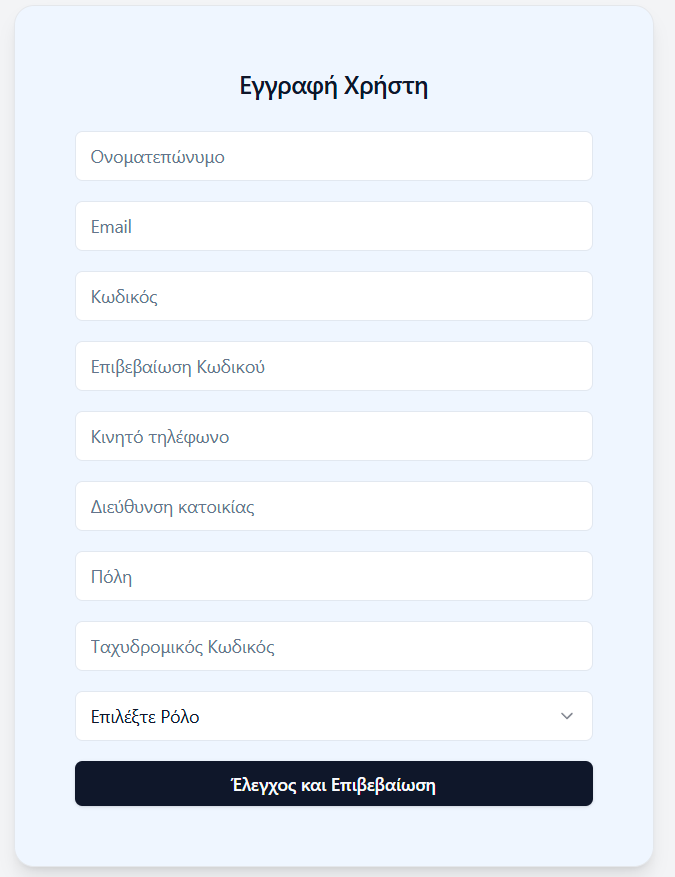
\includegraphics[width=\textwidth]{../Mockup Screens/mockup-register.png}
        \caption{Sign Up Screen}\label{fig:mockup1}
    \end{subfigure}
    \hfill
    \begin{subfigure}[b]{0.48\textwidth}
        \centering
        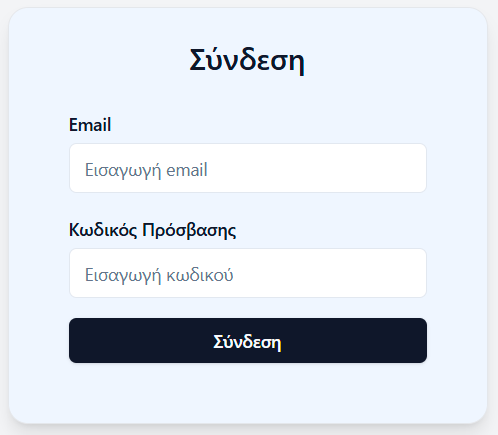
\includegraphics[width=\textwidth]{../Mockup Screens/mockup-login1.png}
        \caption{Sign In Screen}\label{fig:mockup2}
    \end{subfigure}
    \caption{Authentication Screens}\label{fig:auth-screens}
\end{figure}

\begin{figure}[H]
    \centering
    \begin{subfigure}[b]{0.48\textwidth}
        \centering
        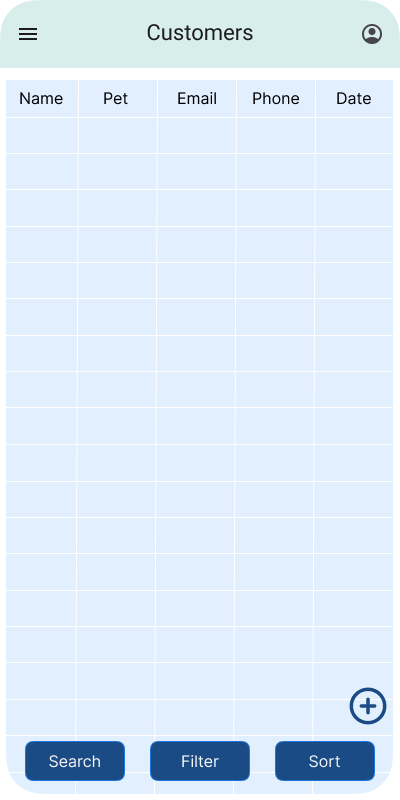
\includegraphics[width=\textwidth,height=0.4\textheight,keepaspectratio]{../Mockup Screens/customer_management.png}
        \caption{Customer Management Screen}\label{fig:mockup3}
    \end{subfigure}
    \hfill
    \begin{subfigure}[b]{0.48\textwidth}
        \centering
        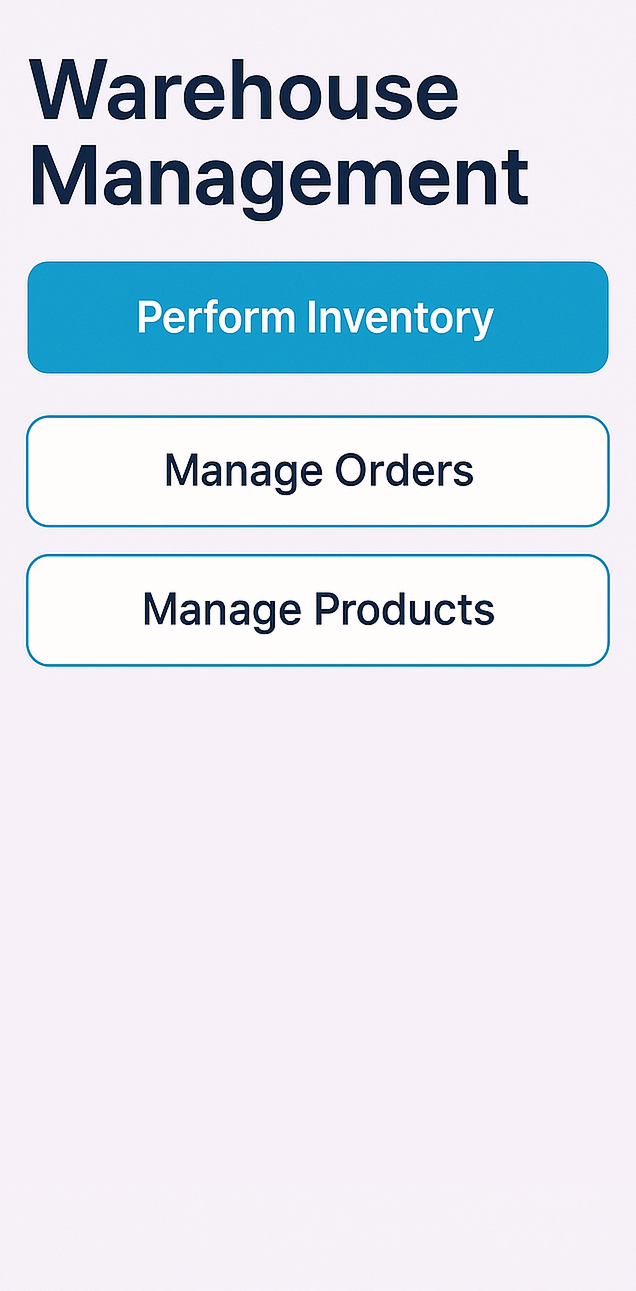
\includegraphics[width=\textwidth,height=0.4\textheight,keepaspectratio]{../Mockup Screens/warehouse_management_products.png}
        \caption{Warehouse Management Screen}\label{fig:mockup4}
    \end{subfigure}
\end{figure}

\begin{figure}[H]
    \centering
    \begin{subfigure}[b]{0.48\textwidth}
        \centering
        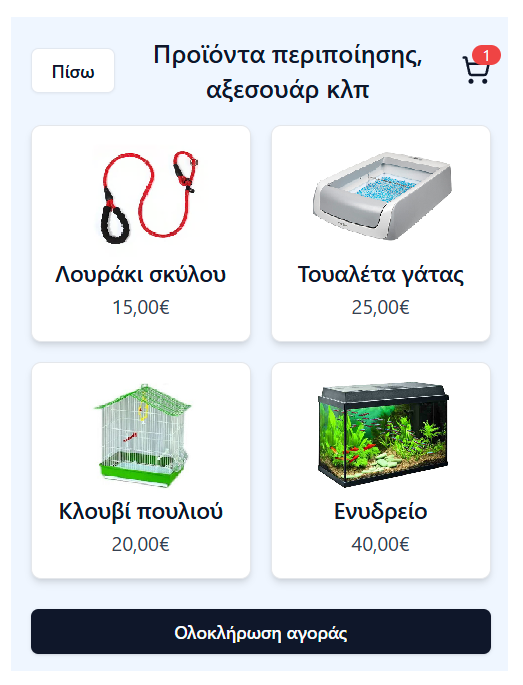
\includegraphics[width=\textwidth]{../Mockup Screens/mockup-store.png}
        \caption{Store Screen}\label{fig:mockup5}
    \end{subfigure}
    \hfill
    \begin{subfigure}[b]{0.48\textwidth}
        \centering
        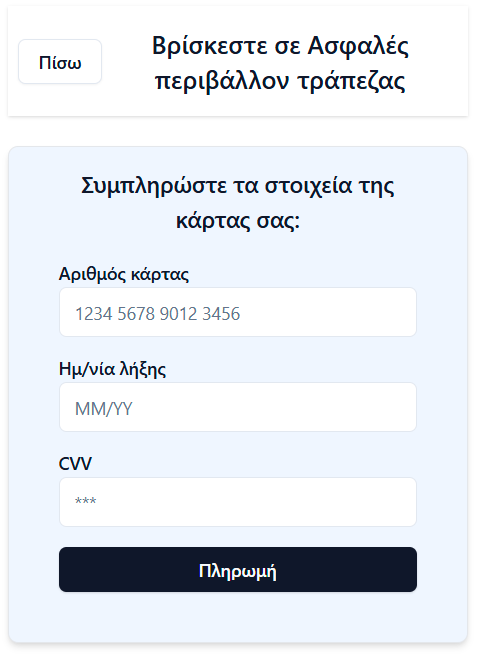
\includegraphics[width=\textwidth]{../Mockup Screens/mockup-payment.png}
        \caption{Payment Screen}\label{fig:mockup6}
    \end{subfigure}
\end{figure}

\begin{figure}[H]
    \centering
    \begin{subfigure}[b]{0.48\textwidth}
        \centering
        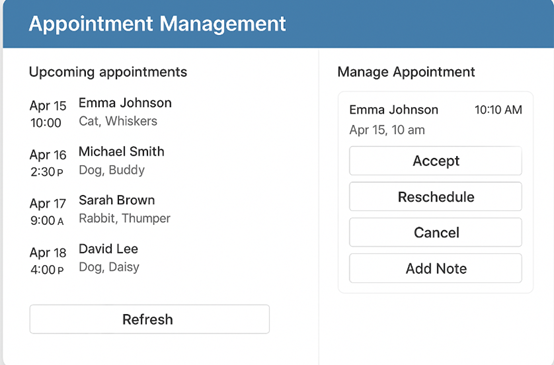
\includegraphics[width=\textwidth]{../Mockup Screens/Appointment_Management.png}
        \caption{Appointment Management Screen}\label{fig:mockup7}
    \end{subfigure}
    \hfill
    \begin{subfigure}[b]{0.48\textwidth}
        \centering
        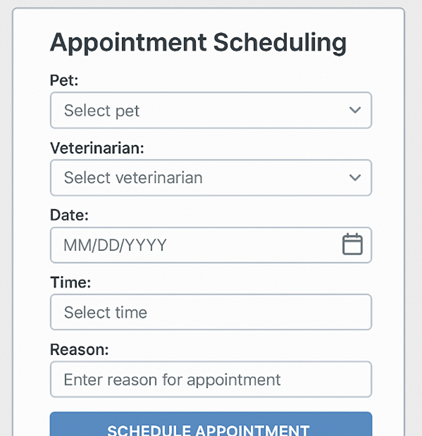
\includegraphics[width=\textwidth]{../Mockup Screens/Appointment_Scheduling.png}
        \caption{Appointment Scheduling Screen}\label{fig:mockup8}
    \end{subfigure}
\end{figure}

\begin{figure}[H]
    \centering
    \begin{subfigure}[b]{0.48\textwidth}
        \centering
        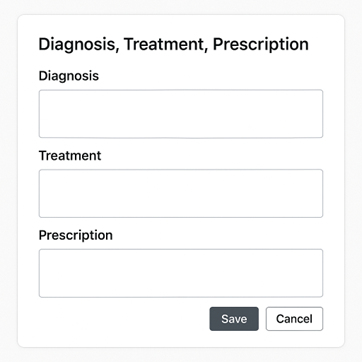
\includegraphics[width=\textwidth]{../Mockup Screens/Diagnosis.png}
        \caption{Medical Record Screen}\label{fig:mockup9}
    \end{subfigure}
    \hfill
    \begin{subfigure}[b]{0.48\textwidth}
        \centering
        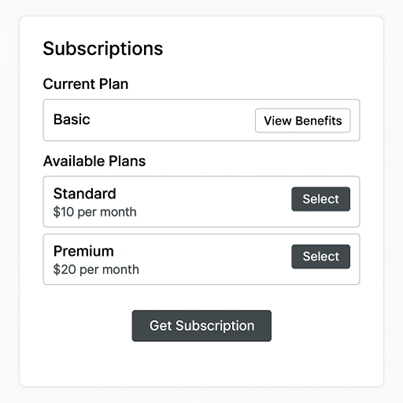
\includegraphics[width=\textwidth]{../Mockup Screens/Subscription.png}
        \caption{Subscriptions Screen}\label{fig:mockup10}
    \end{subfigure}
\end{figure}

\begin{figure}[H]
    \centering
    \begin{subfigure}[b]{0.48\textwidth}
        \centering
        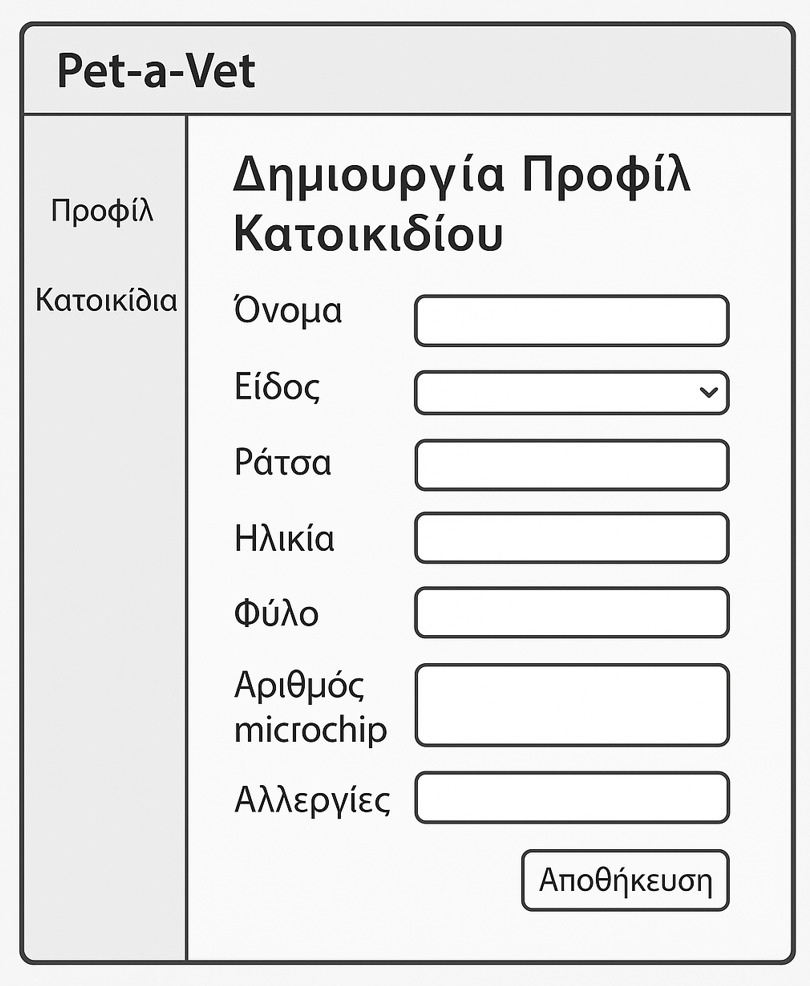
\includegraphics[width=\textwidth]{../Mockup Screens/Pet_profile.png}
        \caption{Profile Creation for Pets Screen}\label{fig:mockup11}
    \end{subfigure}
    \hfill
    \begin{subfigure}[b]{0.48\textwidth}
        \centering
        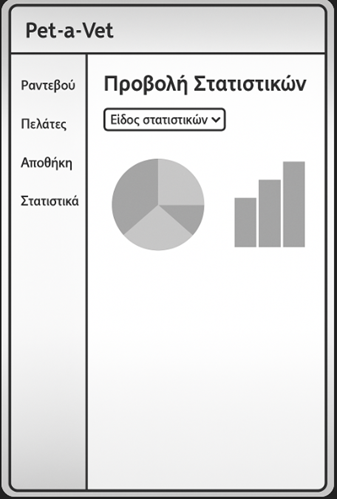
\includegraphics[width=\textwidth]{../Mockup Screens/View_statistics.png}
        \caption{View Statistics Screen}\label{fig:mockup12}
    \end{subfigure}
\end{figure}

\subsection{Παραδοχές} % chktex 19

Χρησιμοποιήθηκε Generative Artificial Intelligence \textit{(Text-to-Image)}, σε συνδυασμό με το εργαλείο \textit{Figma} σε κάποιες περιπτώσεις, για την παραγωγή των παραπάνω οθονών, ενώ σε κάποιες άλλες αναπτύχθηκε σύντομος κώδικας. % chktex 19

\end{document} % chktex 17